 \documentclass{article}
\usepackage[utf8]{inputenc}
\usepackage[a4paper, total={7in, 10in}]{geometry}
\usepackage{braket}
\usepackage{xcolor}
\usepackage{amsmath}
\usepackage{amssymb}
\usepackage{amsfonts}
\usepackage{graphicx}
\usepackage{svg}
\usepackage{float}
\usepackage{tikz}
\usepackage[ruled,vlined]{algorithm2e}
\usepackage{multicol}
\usepackage[backend=biber,style=alphabetic,sorting=ynt]{biblatex}
\usepackage{xcolor}
%\addbibresource{sample.bib} %Import the bibliography file

\newcommand{\commentt}[1]{\textcolor{blue}{ \textbf{[COMMENT]} #1}}
\newcommand{\ctt}[1]{\commentt{#1}}
\newcommand{\prb}[1]{ \mathbf{Pr} \left[ {#1} \right]}
\newcommand{\onotation}[1]{\(\mathcal{O} \left( {#1}  \right) \)}
\newcommand{\ona}[1]{\onotation{#1}}
\newcommand{\PSI}{{\ket{\psi}}}
\newcommand{\LESn}{\ket{\psi_n}}
\newcommand{\LESa}{\ket{\phi_n}}
\newcommand{\LESs}{\frac{1}{\sqrt{n}}\sum_{i}{\ket{\left(0^{i}10^{n-i}\right)^{n}}}}
\newcommand{\Hn}{\mathcal{H}_{n}}
\newcommand{\Ep}{\frac{1}{\sqrt{2^n}}\sum^{2^n}_{x}{ \ket{xx}}}
\newcommand{\HON}{\ket{\psi_{\text{honest}}}}
\newcommand{\Lemma}{\paragraph{Lemma.}}


\setlength{\columnsep}{0.6cm}

\newcommand{\Gz}{ G_{z}^{\delta} } 

\begin{document}

\title{Quantum LTC With Positive Rate}
\author{David Ponarovsky}
\maketitle
%\begin{multicols*}{2}
\newcommand{ \Hw }{ \delta\Delta -\Delta^{\frac{1}{2}-\varepsilon}/\delta  }
	\newcommand{ \Nw }{ \Delta^{\frac{3}{2}-\varepsilon}} 
	  \newcommand{ \Gu } { \Gamma^{\cup} }
	  \newcommand{ \Guq } { \Gamma^{\cup, \square} }

    	\newcommand{ \Gsa } {\Gamma_{\square_{1}} }
	\newcommand{ \Gsb } {\Gamma_{\square_{2}} }
        \newcommand{ \Aa } { C_{A_{1}}}  
	\newcommand{ \Ab } { C_{A_{2}}}
	\newcommand{ \Ac } { C_{A_{3}}}
	\newcommand{ \Aab } { \Aa \otimes \Ab } 
	\newcommand{ \Aac } { \Aa \otimes \Ac }
	\newcommand{ \Aabc } { \Aa \otimes \Ab \otimes \Ac }
	\newcommand{ \Aabp } { \Aa^{\perp} \otimes \Ab^{\perp} } 
	\newcommand{ \Aacp } { \Aa^{\perp} \otimes \Ac^{\perp} }
	\newcommand{ \Aabcp } { \Aa^{\perp} \otimes \Ab^{\perp} \otimes \Ac^{\perp} }
	\newcommand{ \Aabpp } { \left( \Aabp \right)^\perp } 
	\newcommand{ \Aacpp } { \left( \Aacp \right)^\perp }
	\newcommand{ \Aabcpp } { \left( \Aabcp \right)^\perp }
	\newcommand{ \YY } {  y_{1}y_{2}^{\top} }
	\newcommand{ \ZZ } {  z_{1}z_{2}^{\top} } 
	\newcommand{ \TT } { \tilde{\tau} } 


  \paragraph{preamble.} preamble.  
  \begin{figure}[H]
            %\label{fig:square}
            \begin{center}
            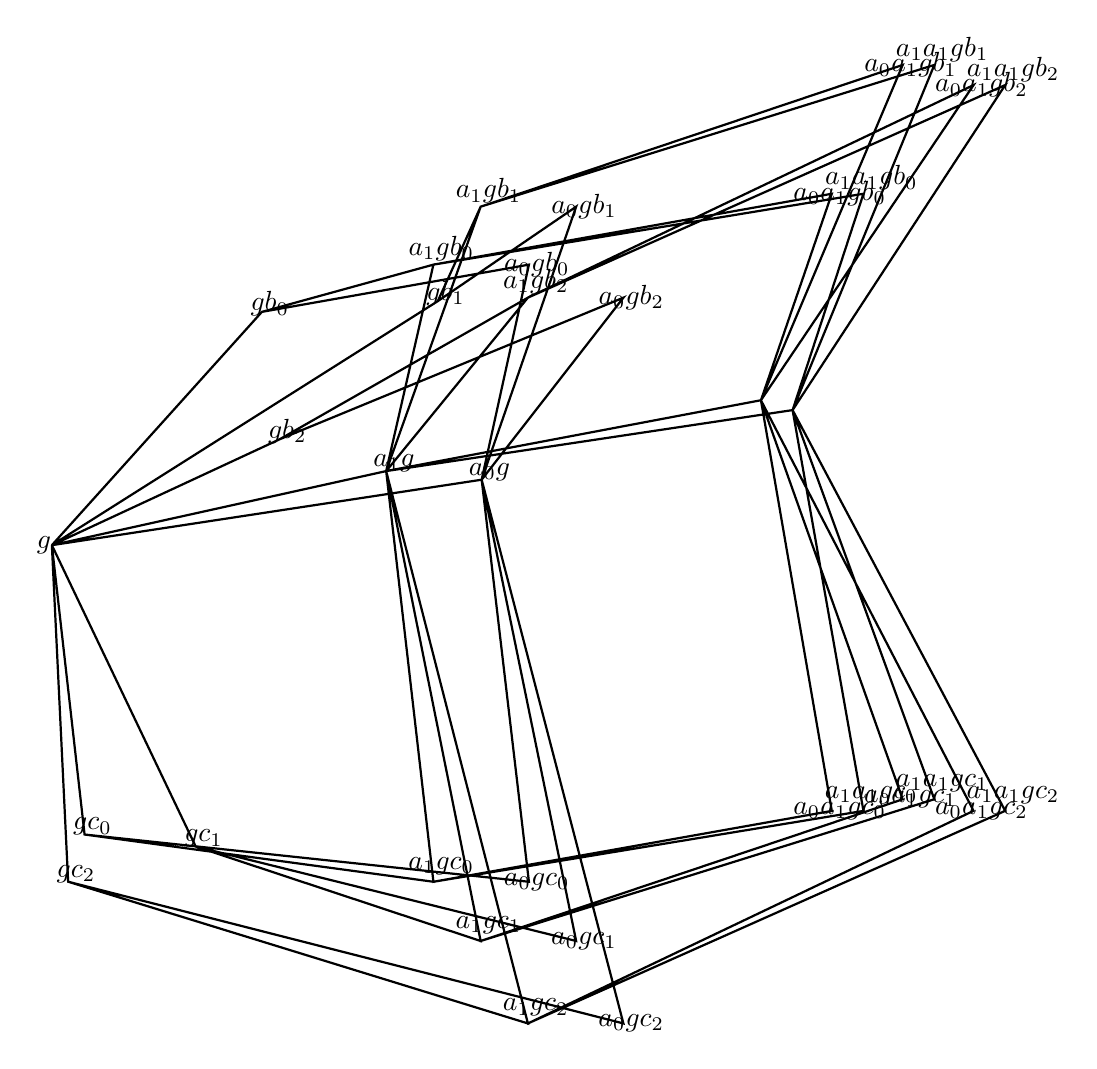
\begin{tikzpicture}
            \draw[thick](0,0)(0, 0) -- (2.6675621315911666,2.962758899993018) -- (6.058461564742955,3.562758899993018) -- (5.458461564742955,0.8312787959571436) -- (0, 0)
(0, 0) -- (4.900833826474292,3.0987982587759424) -- (6.6584615647429555,4.298798258775943) -- (5.458461564742955,0.8312787959571436) -- (0, 0)
(0, 0) -- (2.8896835607956266,1.3432154118855946) -- (7.258461564742955,3.1432154118855946) -- (5.458461564742955,0.8312787959571436) -- (0, 0)
(0, 0) -- (2.6675621315911666,2.962758899993018) -- (4.845592498667492,3.562758899993018) -- (4.245592498667492,0.9407418225254676) -- (0, 0)
(0, 0) -- (4.900833826474292,3.0987982587759424) -- (5.445592498667493,4.298798258775943) -- (4.245592498667492,0.9407418225254676) -- (0, 0)
(0, 0) -- (2.8896835607956266,1.3432154118855946) -- (6.045592498667492,3.1432154118855946) -- (4.245592498667492,0.9407418225254676) -- (0, 0)
(0, 0) -- (0.41548601566723575,-3.674713692941913) -- (6.058461564742955,-4.274713692941913) -- (5.458461564742955,0.8312787959571436) -- (0, 0)
(0, 0) -- (1.826899055028755,-3.8270577423097465) -- (6.6584615647429555,-5.027057742309746) -- (5.458461564742955,0.8312787959571436) -- (0, 0)
(0, 0) -- (0.2066186953388921,-4.27405029083153) -- (7.258461564742955,-6.07405029083153) -- (5.458461564742955,0.8312787959571436) -- (0, 0)
(0, 0) -- (0.41548601566723575,-3.674713692941913) -- (4.845592498667492,-4.274713692941913) -- (4.245592498667492,0.9407418225254676) -- (0, 0)
(0, 0) -- (1.826899055028755,-3.8270577423097465) -- (5.445592498667493,-5.027057742309746) -- (4.245592498667492,0.9407418225254676) -- (0, 0)
(0, 0) -- (0.2066186953388921,-4.27405029083153) -- (6.045592498667492,-6.07405029083153) -- (4.245592498667492,0.9407418225254676) -- (0, 0)
(4.245592498667492, 0.9407418225254676) -- (4.845592498667492,3.562758899993018) -- (9.905239611763031,4.462758899993018) -- (9.005239611763031,1.840485756096379) -- (4.245592498667492, 0.9407418225254676)
(4.245592498667492, 0.9407418225254676) -- (5.445592498667493,4.298798258775943) -- (10.805239611763032,6.098798258775942) -- (9.005239611763031,1.840485756096379) -- (4.245592498667492, 0.9407418225254676)
(4.245592498667492, 0.9407418225254676) -- (6.045592498667492,3.1432154118855946) -- (11.70523961176303,5.843215411885595) -- (9.005239611763031,1.840485756096379) -- (4.245592498667492, 0.9407418225254676)
(4.245592498667492, 0.9407418225254676) -- (4.845592498667492,3.562758899993018) -- (10.307077874478908,4.462758899993018) -- (9.407077874478908,1.7153225442086222) -- (4.245592498667492, 0.9407418225254676)
(4.245592498667492, 0.9407418225254676) -- (5.445592498667493,4.298798258775943) -- (11.207077874478909,6.098798258775942) -- (9.407077874478908,1.7153225442086222) -- (4.245592498667492, 0.9407418225254676)
(4.245592498667492, 0.9407418225254676) -- (6.045592498667492,3.1432154118855946) -- (12.107077874478907,5.843215411885595) -- (9.407077874478908,1.7153225442086222) -- (4.245592498667492, 0.9407418225254676)
(4.245592498667492, 0.9407418225254676) -- (4.845592498667492,-4.274713692941913) -- (9.905239611763031,-3.374713692941913) -- (9.005239611763031,1.840485756096379) -- (4.245592498667492, 0.9407418225254676)
(4.245592498667492, 0.9407418225254676) -- (5.445592498667493,-5.027057742309746) -- (10.805239611763032,-3.2270577423097464) -- (9.005239611763031,1.840485756096379) -- (4.245592498667492, 0.9407418225254676)
(4.245592498667492, 0.9407418225254676) -- (6.045592498667492,-6.07405029083153) -- (11.70523961176303,-3.37405029083153) -- (9.005239611763031,1.840485756096379) -- (4.245592498667492, 0.9407418225254676)
(4.245592498667492, 0.9407418225254676) -- (4.845592498667492,-4.274713692941913) -- (10.307077874478908,-3.374713692941913) -- (9.407077874478908,1.7153225442086222) -- (4.245592498667492, 0.9407418225254676)
(4.245592498667492, 0.9407418225254676) -- (5.445592498667493,-5.027057742309746) -- (11.207077874478909,-3.2270577423097464) -- (9.407077874478908,1.7153225442086222) -- (4.245592498667492, 0.9407418225254676)
(4.245592498667492, 0.9407418225254676) -- (6.045592498667492,-6.07405029083153) -- (12.107077874478907,-3.37405029083153) -- (9.407077874478908,1.7153225442086222) -- (4.245592498667492, 0.9407418225254676)
;
\node at (6.158461564742955,3.562758899993018) {$ a_{ 0  } gb_{ 0 } $};
\node at (6.758461564742955,4.298798258775943) {$ a_{ 0  } gb_{ 1 } $};
\node at (7.358461564742955,3.1432154118855946) {$ a_{ 0  } gb_{ 2 } $};
\node at (4.945592498667492,3.762758899993018) {$ a_{ 1  } gb_{ 0 } $};
\node at (5.545592498667492,4.498798258775943) {$ a_{ 1  } gb_{ 1 } $};
\node at (6.145592498667492,3.343215411885595) {$ a_{ 1  } gb_{ 2 } $};
\node at (6.158461564742955,-4.274713692941913) {$ a_{ 0  } gc_{ 0 } $};
\node at (6.758461564742955,-5.027057742309746) {$ a_{ 0  } gc_{ 1 } $};
\node at (7.358461564742955,-6.07405029083153) {$ a_{ 0  } gc_{ 2 } $};
\node at (4.945592498667492,-4.074713692941913) {$ a_{ 1  } gc_{ 0 } $};
\node at (5.545592498667492,-4.827057742309746) {$ a_{ 1  } gc_{ 1 } $};
\node at (6.145592498667492,-5.87405029083153) {$ a_{ 1  } gc_{ 2 } $};
\node at (10.005239611763031,4.462758899993018) {$ a_{ 0  } a_{ 1 }gb_{ 0 } $};
\node at (10.905239611763031,6.098798258775942) {$ a_{ 0  } a_{ 1 }gb_{ 1 } $};
\node at (11.80523961176303,5.843215411885595) {$ a_{ 0  } a_{ 1 }gb_{ 2 } $};
\node at (10.407077874478908,4.662758899993018) {$ a_{ 1  } a_{ 1 }gb_{ 0 } $};
\node at (11.307077874478908,6.298798258775943) {$ a_{ 1  } a_{ 1 }gb_{ 1 } $};
\node at (12.207077874478907,6.043215411885595) {$ a_{ 1  } a_{ 1 }gb_{ 2 } $};
\node at (10.005239611763031,-3.374713692941913) {$ a_{ 0  } a_{ 1 }gc_{ 0 } $};
\node at (10.905239611763031,-3.2270577423097464) {$ a_{ 0  } a_{ 1 }gc_{ 1 } $};
\node at (11.80523961176303,-3.37405029083153) {$ a_{ 0  } a_{ 1 }gc_{ 2 } $};
\node at (10.407077874478908,-3.174713692941913) {$ a_{ 1  } a_{ 1 }gc_{ 0 } $};
\node at (11.307077874478908,-3.0270577423097462) {$ a_{ 1  } a_{ 1 }gc_{ 1 } $};
\node at (12.207077874478907,-3.17405029083153) {$ a_{ 1  } a_{ 1 }gc_{ 2 } $};
\node at (-0.1,0) {$ g $};
\node at (5.558461564742955,0.9312787959571436) {$ a_{ 0 }g $};
\node at (4.345592498667492,1.0407418225254677) {$ a_{ 1 }g $};
\node at (2.7675621315911667,3.062758899993018) {$ gb_{ 0 } $};
\node at (5.000833826474292,3.1987982587759425) {$ gb_{ 1 } $};
\node at (2.9896835607956267,1.4432154118855947) {$ gb_{ 2 } $};
\node at (0.5154860156672357,-3.5747136929419128) {$ gc_{ 0 } $};
\node at (1.926899055028755,-3.7270577423097464) {$ gc_{ 1 } $};
\node at (0.3066186953388921,-4.174050290831531) {$ gc_{ 2 } $};

            \end{tikzpicture}
            \end{center}
            \caption{Square of the complex, with edges $(g,ag), (agb, gb) \in E_A,
            (g,gb), (agb, ag) \in E_B.$ \label{fig:square}
            }
            \end{figure}
 \begin{figure}[H]
            %\label{fig:square}
            \begin{center}
            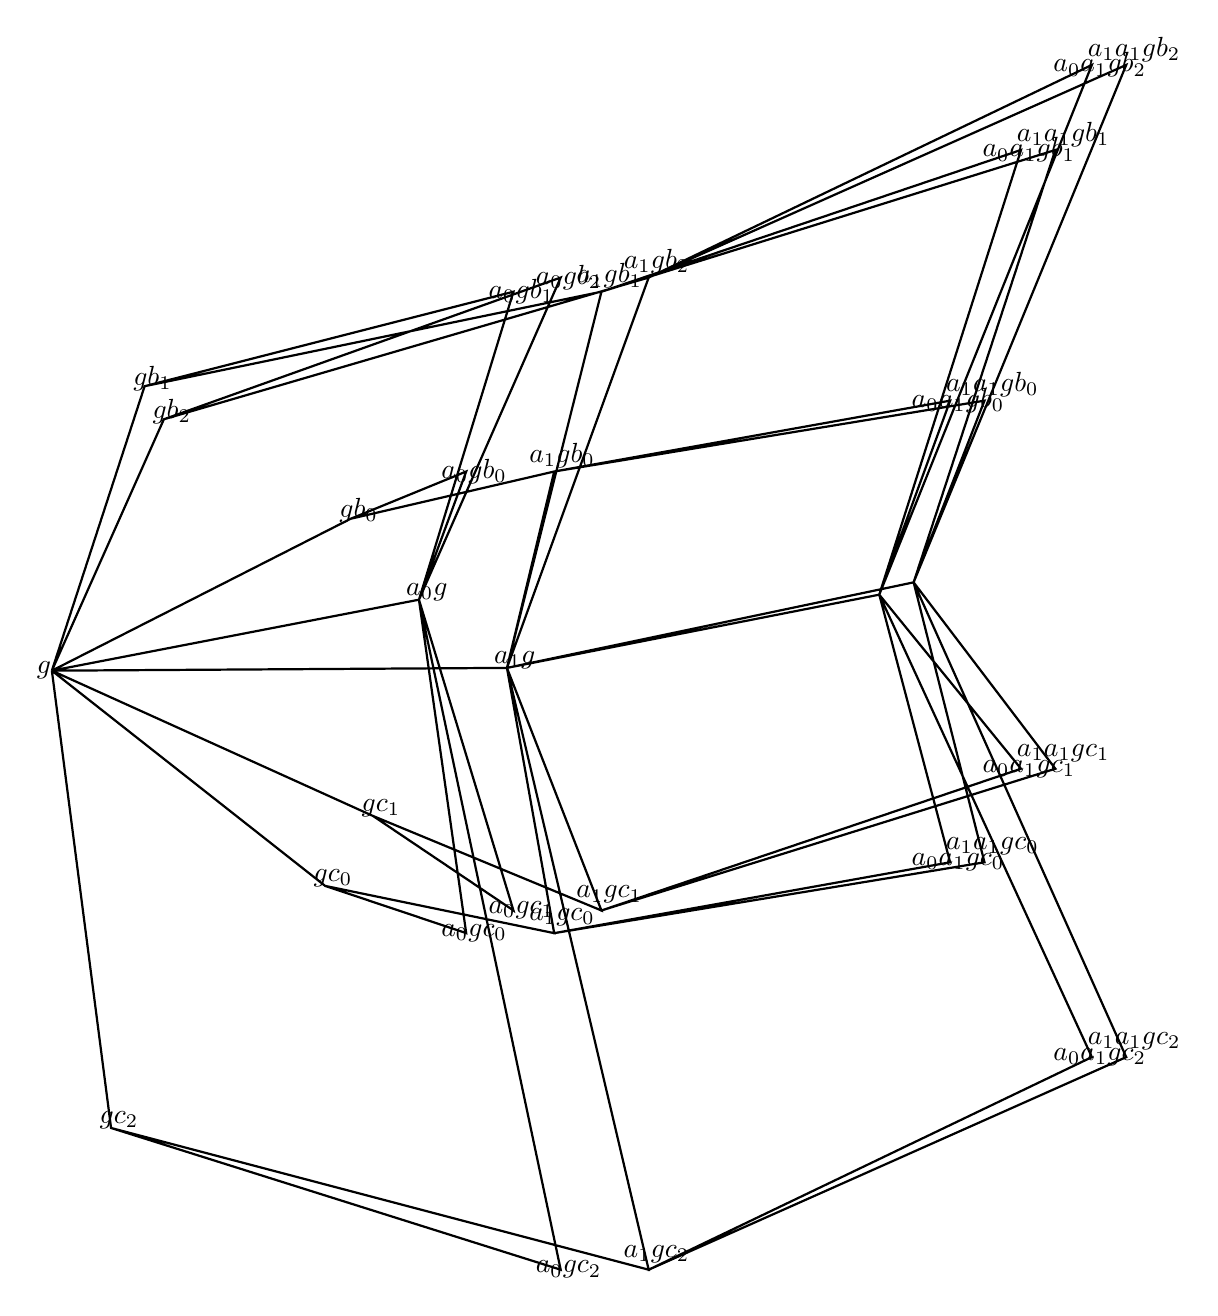
\begin{tikzpicture}
            \draw[thick](0,0)(0, 0) -- (3.7951057076096784,1.9292503870353819) -- (5.262030930408452,2.5292503870353817) -- (4.662030930408452,0.9013132379642899) -- (0, 0)
(0, 0) -- (1.1779609695681015,3.6128184361140843) -- (5.862030930408452,4.812818436114084) -- (4.662030930408452,0.9013132379642899) -- (0, 0)
(0, 0) -- (1.4223982622929983,3.1927285987895333) -- (6.462030930408452,4.992728598789533) -- (4.662030930408452,0.9013132379642899) -- (0, 0)
(0, 0) -- (3.7951057076096784,1.9292503870353819) -- (6.37947686718632,2.5292503870353817) -- (5.77947686718632,0.03517839577285007) -- (0, 0)
(0, 0) -- (1.1779609695681015,3.6128184361140843) -- (6.97947686718632,4.812818436114084) -- (5.77947686718632,0.03517839577285007) -- (0, 0)
(0, 0) -- (1.4223982622929983,3.1927285987895333) -- (7.57947686718632,4.992728598789533) -- (5.77947686718632,0.03517839577285007) -- (0, 0)
(0, 0) -- (3.4708583019717203,-2.733387243147641) -- (5.262030930408452,-3.3333872431476412) -- (4.662030930408452,0.9013132379642899) -- (0, 0)
(0, 0) -- (4.078932180783047,-1.8454432125467826) -- (5.862030930408452,-3.0454432125467825) -- (4.662030930408452,0.9013132379642899) -- (0, 0)
(0, 0) -- (0.7519392290473637,-5.807649374937764) -- (6.462030930408452,-7.607649374937764) -- (4.662030930408452,0.9013132379642899) -- (0, 0)
(0, 0) -- (3.4708583019717203,-2.733387243147641) -- (6.37947686718632,-3.3333872431476412) -- (5.77947686718632,0.03517839577285007) -- (0, 0)
(0, 0) -- (4.078932180783047,-1.8454432125467826) -- (6.97947686718632,-3.0454432125467825) -- (5.77947686718632,0.03517839577285007) -- (0, 0)
(0, 0) -- (0.7519392290473637,-5.807649374937764) -- (7.57947686718632,-7.607649374937764) -- (5.77947686718632,0.03517839577285007) -- (0, 0)
(5.77947686718632, 0.03517839577285007) -- (6.37947686718632,2.5292503870353817) -- (11.407916131426203,3.4292503870353817) -- (10.507916131426203,0.9653707932252876) -- (5.77947686718632, 0.03517839577285007)
(5.77947686718632, 0.03517839577285007) -- (6.97947686718632,4.812818436114084) -- (12.307916131426204,6.612818436114084) -- (10.507916131426203,0.9653707932252876) -- (5.77947686718632, 0.03517839577285007)
(5.77947686718632, 0.03517839577285007) -- (7.57947686718632,4.992728598789533) -- (13.207916131426202,7.692728598789533) -- (10.507916131426203,0.9653707932252876) -- (5.77947686718632, 0.03517839577285007)
(5.77947686718632, 0.03517839577285007) -- (6.37947686718632,2.5292503870353817) -- (11.84415629535483,3.4292503870353817) -- (10.94415629535483,1.1216627447186642) -- (5.77947686718632, 0.03517839577285007)
(5.77947686718632, 0.03517839577285007) -- (6.97947686718632,4.812818436114084) -- (12.74415629535483,6.612818436114084) -- (10.94415629535483,1.1216627447186642) -- (5.77947686718632, 0.03517839577285007)
(5.77947686718632, 0.03517839577285007) -- (7.57947686718632,4.992728598789533) -- (13.64415629535483,7.692728598789533) -- (10.94415629535483,1.1216627447186642) -- (5.77947686718632, 0.03517839577285007)
(5.77947686718632, 0.03517839577285007) -- (6.37947686718632,-3.3333872431476412) -- (11.407916131426203,-2.4333872431476413) -- (10.507916131426203,0.9653707932252876) -- (5.77947686718632, 0.03517839577285007)
(5.77947686718632, 0.03517839577285007) -- (6.97947686718632,-3.0454432125467825) -- (12.307916131426204,-1.2454432125467825) -- (10.507916131426203,0.9653707932252876) -- (5.77947686718632, 0.03517839577285007)
(5.77947686718632, 0.03517839577285007) -- (7.57947686718632,-7.607649374937764) -- (13.207916131426202,-4.907649374937764) -- (10.507916131426203,0.9653707932252876) -- (5.77947686718632, 0.03517839577285007)
(5.77947686718632, 0.03517839577285007) -- (6.37947686718632,-3.3333872431476412) -- (11.84415629535483,-2.4333872431476413) -- (10.94415629535483,1.1216627447186642) -- (5.77947686718632, 0.03517839577285007)
(5.77947686718632, 0.03517839577285007) -- (6.97947686718632,-3.0454432125467825) -- (12.74415629535483,-1.2454432125467825) -- (10.94415629535483,1.1216627447186642) -- (5.77947686718632, 0.03517839577285007)
(5.77947686718632, 0.03517839577285007) -- (7.57947686718632,-7.607649374937764) -- (13.64415629535483,-4.907649374937764) -- (10.94415629535483,1.1216627447186642) -- (5.77947686718632, 0.03517839577285007)
;
\node at (5.3620309304084515,2.5292503870353817) {$ a_{ 0  } gb_{ 0 } $};
\node at (5.962030930408452,4.812818436114084) {$ a_{ 0  } gb_{ 1 } $};
\node at (6.562030930408452,4.992728598789533) {$ a_{ 0  } gb_{ 2 } $};
\node at (6.479476867186319,2.729250387035382) {$ a_{ 1  } gb_{ 0 } $};
\node at (7.07947686718632,5.012818436114085) {$ a_{ 1  } gb_{ 1 } $};
\node at (7.679476867186319,5.192728598789533) {$ a_{ 1  } gb_{ 2 } $};
\node at (5.3620309304084515,-3.3333872431476412) {$ a_{ 0  } gc_{ 0 } $};
\node at (5.962030930408452,-3.0454432125467825) {$ a_{ 0  } gc_{ 1 } $};
\node at (6.562030930408452,-7.607649374937764) {$ a_{ 0  } gc_{ 2 } $};
\node at (6.479476867186319,-3.133387243147641) {$ a_{ 1  } gc_{ 0 } $};
\node at (7.07947686718632,-2.8454432125467823) {$ a_{ 1  } gc_{ 1 } $};
\node at (7.679476867186319,-7.407649374937764) {$ a_{ 1  } gc_{ 2 } $};
\node at (11.507916131426203,3.4292503870353817) {$ a_{ 0  } a_{ 1 }gb_{ 0 } $};
\node at (12.407916131426203,6.612818436114084) {$ a_{ 0  } a_{ 1 }gb_{ 1 } $};
\node at (13.307916131426202,7.692728598789533) {$ a_{ 0  } a_{ 1 }gb_{ 2 } $};
\node at (11.94415629535483,3.629250387035382) {$ a_{ 1  } a_{ 1 }gb_{ 0 } $};
\node at (12.84415629535483,6.812818436114084) {$ a_{ 1  } a_{ 1 }gb_{ 1 } $};
\node at (13.744156295354829,7.8927285987895335) {$ a_{ 1  } a_{ 1 }gb_{ 2 } $};
\node at (11.507916131426203,-2.4333872431476413) {$ a_{ 0  } a_{ 1 }gc_{ 0 } $};
\node at (12.407916131426203,-1.2454432125467825) {$ a_{ 0  } a_{ 1 }gc_{ 1 } $};
\node at (13.307916131426202,-4.907649374937764) {$ a_{ 0  } a_{ 1 }gc_{ 2 } $};
\node at (11.94415629535483,-2.233387243147641) {$ a_{ 1  } a_{ 1 }gc_{ 0 } $};
\node at (12.84415629535483,-1.0454432125467825) {$ a_{ 1  } a_{ 1 }gc_{ 1 } $};
\node at (13.744156295354829,-4.7076493749377635) {$ a_{ 1  } a_{ 1 }gc_{ 2 } $};
\node at (-0.1,0) {$ g $};
\node at (4.762030930408452,1.00131323796429) {$ a_{ 0 }g $};
\node at (5.87947686718632,0.13517839577285007) {$ a_{ 1 }g $};
\node at (3.8951057076096784,2.0292503870353817) {$ gb_{ 0 } $};
\node at (1.2779609695681016,3.7128184361140844) {$ gb_{ 1 } $};
\node at (1.5223982622929983,3.2927285987895334) {$ gb_{ 2 } $};
\node at (3.5708583019717204,-2.633387243147641) {$ gc_{ 0 } $};
\node at (4.178932180783047,-1.7454432125467825) {$ gc_{ 1 } $};
\node at (0.8519392290473636,-5.707649374937764) {$ gc_{ 2 } $};

            \end{tikzpicture}
            \end{center}
            \caption{Square of the complex, with edges $(g,ag), (agb, gb) \in E_A,
            (g,gb), (agb, ag) \in E_B.$ \label{fig:square}
            }
            \end{figure}
 \begin{figure}[H]
            %\label{fig:square}
            \begin{center}
            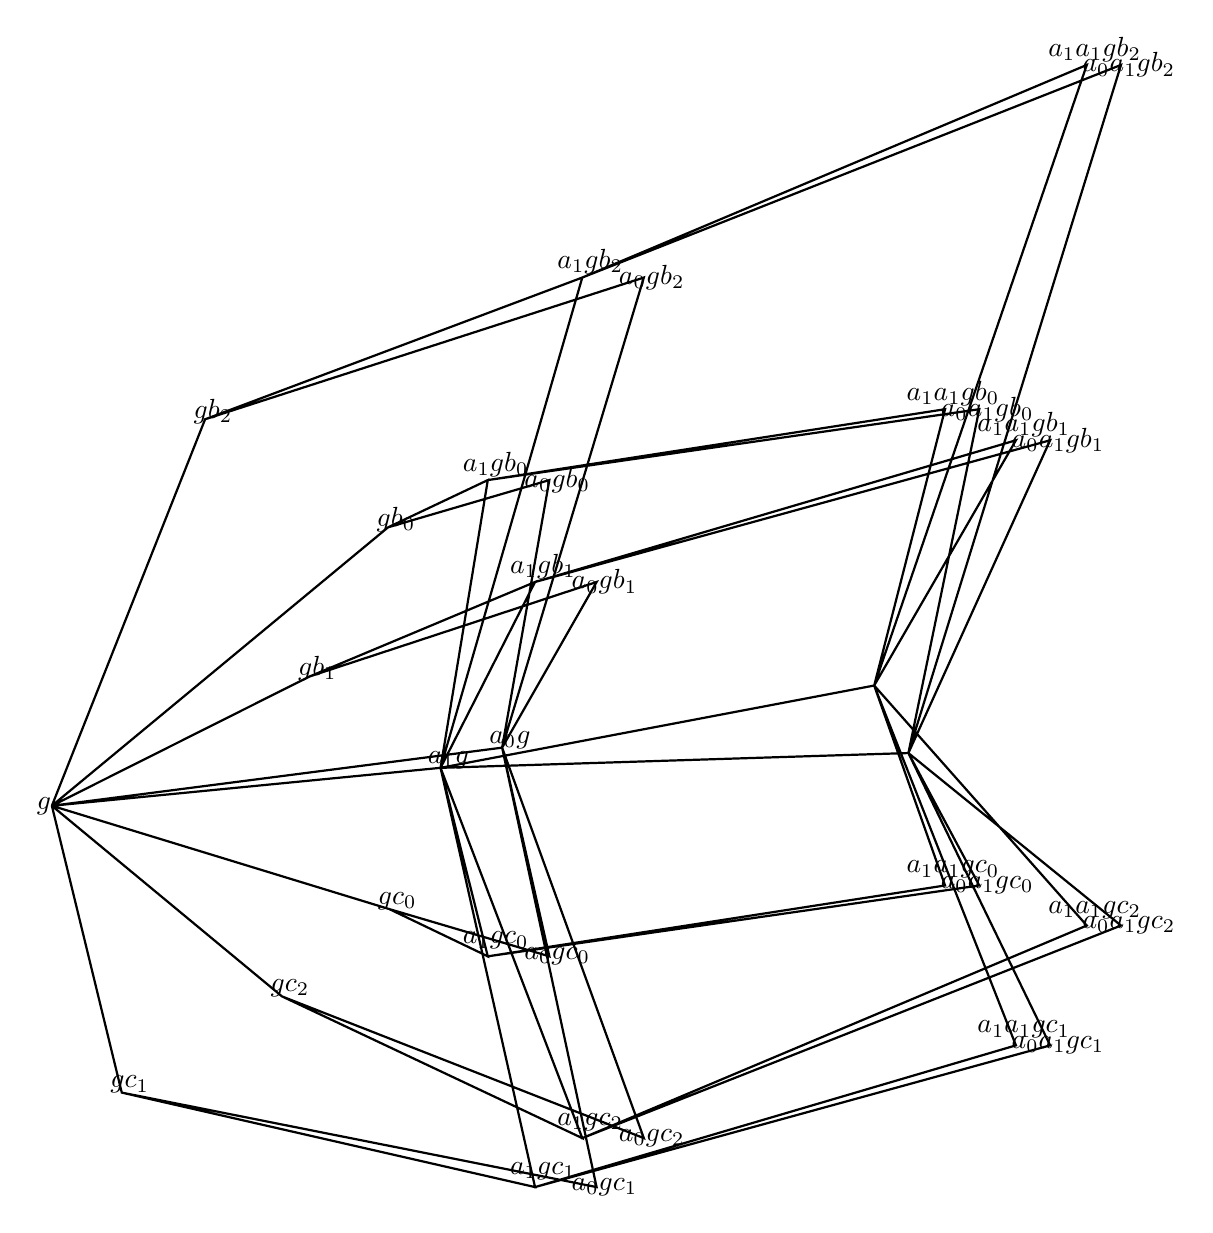
\begin{tikzpicture}
            \draw[thick](0,0)(0, 0) -- (4.269708132442359,3.5361712820805025) -- (6.318024540718383,4.136171282080502) -- (5.718024540718384,0.738118103886632) -- (0, 0)
(0, 0) -- (3.272514185880753,1.6418243702959592) -- (6.918024540718384,2.841824370295959) -- (5.718024540718384,0.738118103886632) -- (0, 0)
(0, 0) -- (1.9462276905191889,4.908530494286637) -- (7.518024540718383,6.708530494286637) -- (5.718024540718384,0.738118103886632) -- (0, 0)
(0, 0) -- (4.269708132442359,3.5361712820805025) -- (5.53629993187062,4.136171282080502) -- (4.936299931870621,0.4817979498012552) -- (0, 0)
(0, 0) -- (3.272514185880753,1.6418243702959592) -- (6.136299931870621,2.841824370295959) -- (4.936299931870621,0.4817979498012552) -- (0, 0)
(0, 0) -- (1.9462276905191889,4.908530494286637) -- (6.7362999318706205,6.708530494286637) -- (4.936299931870621,0.4817979498012552) -- (0, 0)
(0, 0) -- (4.286022249927479,-1.3121565581182977) -- (6.318024540718383,-1.9121565581182978) -- (5.718024540718384,0.738118103886632) -- (0, 0)
(0, 0) -- (0.8879207549031615,-3.6426291881903996) -- (6.918024540718384,-4.8426291881904) -- (5.718024540718384,0.738118103886632) -- (0, 0)
(0, 0) -- (2.922811309833955,-2.420968883609633) -- (7.518024540718383,-4.220968883609633) -- (5.718024540718384,0.738118103886632) -- (0, 0)
(0, 0) -- (4.286022249927479,-1.3121565581182977) -- (5.53629993187062,-1.9121565581182978) -- (4.936299931870621,0.4817979498012552) -- (0, 0)
(0, 0) -- (0.8879207549031615,-3.6426291881903996) -- (6.136299931870621,-4.8426291881904) -- (4.936299931870621,0.4817979498012552) -- (0, 0)
(0, 0) -- (2.922811309833955,-2.420968883609633) -- (6.7362999318706205,-4.220968883609633) -- (4.936299931870621,0.4817979498012552) -- (0, 0)
(4.936299931870621, 0.4817979498012552) -- (5.53629993187062,4.136171282080502) -- (11.777909790768684,5.0361712820805025) -- (10.877909790768683,0.6695651369586144) -- (4.936299931870621, 0.4817979498012552)
(4.936299931870621, 0.4817979498012552) -- (6.136299931870621,2.841824370295959) -- (12.677909790768684,4.641824370295959) -- (10.877909790768683,0.6695651369586144) -- (4.936299931870621, 0.4817979498012552)
(4.936299931870621, 0.4817979498012552) -- (6.7362999318706205,6.708530494286637) -- (13.577909790768683,9.408530494286637) -- (10.877909790768683,0.6695651369586144) -- (4.936299931870621, 0.4817979498012552)
(4.936299931870621, 0.4817979498012552) -- (5.53629993187062,4.136171282080502) -- (11.343320240750588,5.0361712820805025) -- (10.443320240750587,1.5270017650970966) -- (4.936299931870621, 0.4817979498012552)
(4.936299931870621, 0.4817979498012552) -- (6.136299931870621,2.841824370295959) -- (12.243320240750588,4.641824370295959) -- (10.443320240750587,1.5270017650970966) -- (4.936299931870621, 0.4817979498012552)
(4.936299931870621, 0.4817979498012552) -- (6.7362999318706205,6.708530494286637) -- (13.143320240750587,9.408530494286637) -- (10.443320240750587,1.5270017650970966) -- (4.936299931870621, 0.4817979498012552)
(4.936299931870621, 0.4817979498012552) -- (5.53629993187062,-1.9121565581182978) -- (11.777909790768684,-1.0121565581182979) -- (10.877909790768683,0.6695651369586144) -- (4.936299931870621, 0.4817979498012552)
(4.936299931870621, 0.4817979498012552) -- (6.136299931870621,-4.8426291881904) -- (12.677909790768684,-3.0426291881904) -- (10.877909790768683,0.6695651369586144) -- (4.936299931870621, 0.4817979498012552)
(4.936299931870621, 0.4817979498012552) -- (6.7362999318706205,-4.220968883609633) -- (13.577909790768683,-1.5209688836096324) -- (10.877909790768683,0.6695651369586144) -- (4.936299931870621, 0.4817979498012552)
(4.936299931870621, 0.4817979498012552) -- (5.53629993187062,-1.9121565581182978) -- (11.343320240750588,-1.0121565581182979) -- (10.443320240750587,1.5270017650970966) -- (4.936299931870621, 0.4817979498012552)
(4.936299931870621, 0.4817979498012552) -- (6.136299931870621,-4.8426291881904) -- (12.243320240750588,-3.0426291881904) -- (10.443320240750587,1.5270017650970966) -- (4.936299931870621, 0.4817979498012552)
(4.936299931870621, 0.4817979498012552) -- (6.7362999318706205,-4.220968883609633) -- (13.143320240750587,-1.5209688836096324) -- (10.443320240750587,1.5270017650970966) -- (4.936299931870621, 0.4817979498012552)
;
\node at (6.418024540718383,4.136171282080502) {$ a_{ 0  } gb_{ 0 } $};
\node at (7.018024540718383,2.841824370295959) {$ a_{ 0  } gb_{ 1 } $};
\node at (7.618024540718383,6.708530494286637) {$ a_{ 0  } gb_{ 2 } $};
\node at (5.63629993187062,4.336171282080502) {$ a_{ 1  } gb_{ 0 } $};
\node at (6.2362999318706205,3.0418243702959593) {$ a_{ 1  } gb_{ 1 } $};
\node at (6.83629993187062,6.908530494286637) {$ a_{ 1  } gb_{ 2 } $};
\node at (6.418024540718383,-1.9121565581182978) {$ a_{ 0  } gc_{ 0 } $};
\node at (7.018024540718383,-4.8426291881904) {$ a_{ 0  } gc_{ 1 } $};
\node at (7.618024540718383,-4.220968883609633) {$ a_{ 0  } gc_{ 2 } $};
\node at (5.63629993187062,-1.7121565581182978) {$ a_{ 1  } gc_{ 0 } $};
\node at (6.2362999318706205,-4.6426291881904) {$ a_{ 1  } gc_{ 1 } $};
\node at (6.83629993187062,-4.0209688836096324) {$ a_{ 1  } gc_{ 2 } $};
\node at (11.877909790768683,5.0361712820805025) {$ a_{ 0  } a_{ 1 }gb_{ 0 } $};
\node at (12.777909790768684,4.641824370295959) {$ a_{ 0  } a_{ 1 }gb_{ 1 } $};
\node at (13.677909790768682,9.408530494286637) {$ a_{ 0  } a_{ 1 }gb_{ 2 } $};
\node at (11.443320240750587,5.236171282080503) {$ a_{ 1  } a_{ 1 }gb_{ 0 } $};
\node at (12.343320240750588,4.841824370295959) {$ a_{ 1  } a_{ 1 }gb_{ 1 } $};
\node at (13.243320240750586,9.608530494286637) {$ a_{ 1  } a_{ 1 }gb_{ 2 } $};
\node at (11.877909790768683,-1.0121565581182979) {$ a_{ 0  } a_{ 1 }gc_{ 0 } $};
\node at (12.777909790768684,-3.0426291881904) {$ a_{ 0  } a_{ 1 }gc_{ 1 } $};
\node at (13.677909790768682,-1.5209688836096324) {$ a_{ 0  } a_{ 1 }gc_{ 2 } $};
\node at (11.443320240750587,-0.8121565581182979) {$ a_{ 1  } a_{ 1 }gc_{ 0 } $};
\node at (12.343320240750588,-2.8426291881904) {$ a_{ 1  } a_{ 1 }gc_{ 1 } $};
\node at (13.243320240750586,-1.3209688836096325) {$ a_{ 1  } a_{ 1 }gc_{ 2 } $};
\node at (-0.1,0) {$ g $};
\node at (5.818024540718383,0.838118103886632) {$ a_{ 0 }g $};
\node at (5.03629993187062,0.5817979498012552) {$ a_{ 1 }g $};
\node at (4.369708132442359,3.6361712820805026) {$ gb_{ 0 } $};
\node at (3.3725141858807532,1.7418243702959593) {$ gb_{ 1 } $};
\node at (2.046227690519189,5.008530494286637) {$ gb_{ 2 } $};
\node at (4.386022249927478,-1.2121565581182976) {$ gc_{ 0 } $};
\node at (0.9879207549031614,-3.5426291881903995) {$ gc_{ 1 } $};
\node at (3.0228113098339553,-2.3209688836096327) {$ gc_{ 2 } $};

            \end{tikzpicture}
            \end{center}
            \caption{Square of the complex, with edges $(g,ag), (agb, gb) \in E_A,
            (g,gb), (agb, ag) \in E_B.$ \label{fig:square}
            }
            \end{figure}
 \begin{figure}[H]
            %\label{fig:square}
            \begin{center}
            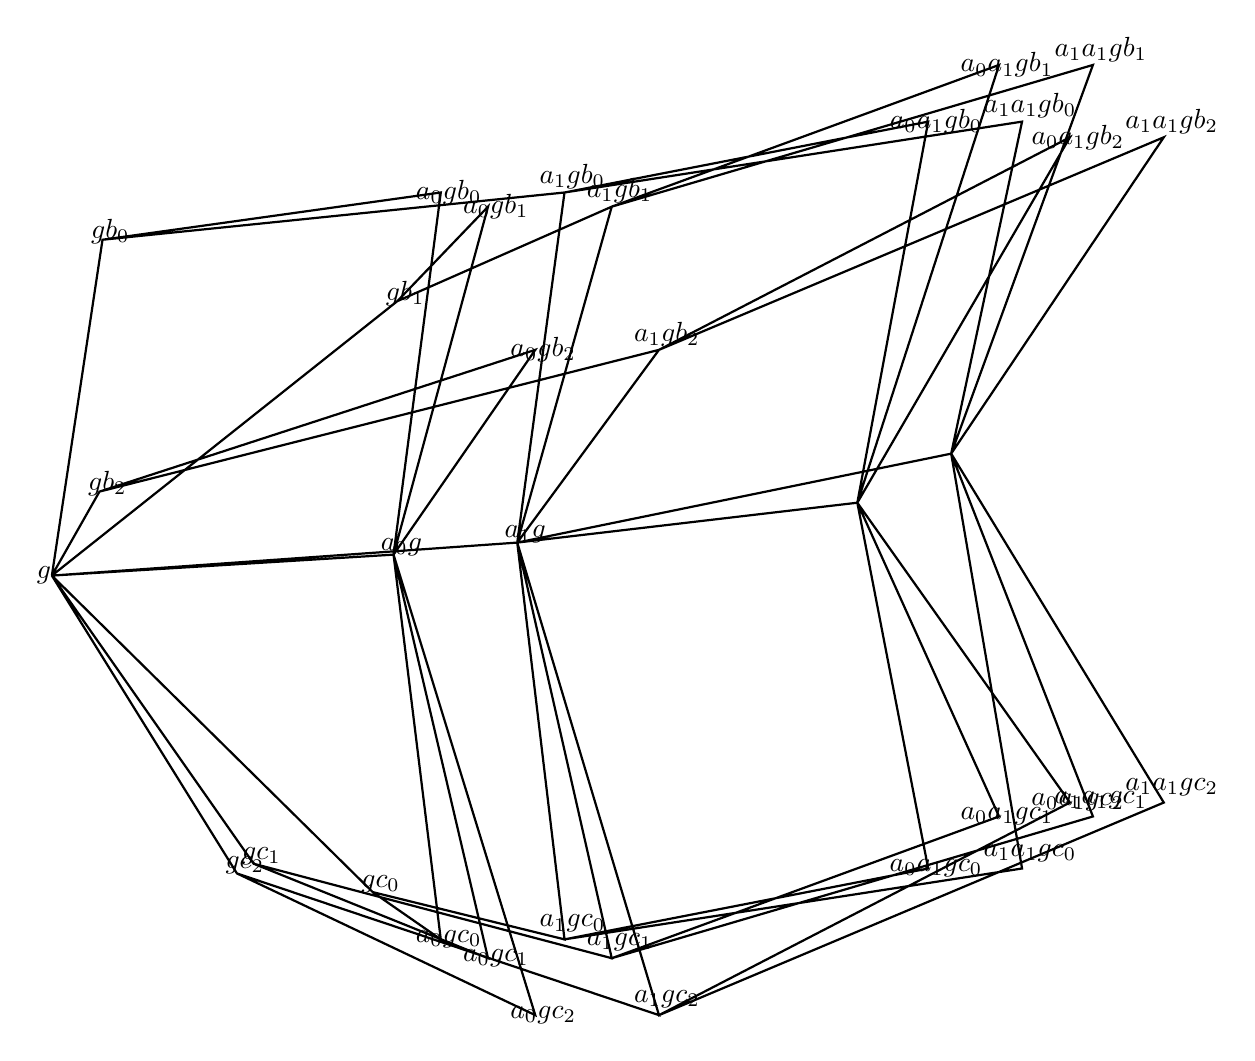
\begin{tikzpicture}
            \draw[thick](0,0)(0, 0) -- (0.643216587490264,4.265324944196854) -- (4.939166826480127,4.865324944196853) -- (4.3391668264801275,0.266171517070706) -- (0, 0)
(0, 0) -- (4.3870439303216475,3.4853248133267183) -- (5.539166826480128,4.6853248133267185) -- (4.3391668264801275,0.266171517070706) -- (0, 0)
(0, 0) -- (0.604680958855226,1.0668088303533831) -- (6.139166826480127,2.866808830353383) -- (4.3391668264801275,0.266171517070706) -- (0, 0)
(0, 0) -- (0.643216587490264,4.265324944196854) -- (6.510356195851917,4.865324944196853) -- (5.910356195851917,0.41930023915271436) -- (0, 0)
(0, 0) -- (4.3870439303216475,3.4853248133267183) -- (7.110356195851917,4.6853248133267185) -- (5.910356195851917,0.41930023915271436) -- (0, 0)
(0, 0) -- (0.604680958855226,1.0668088303533831) -- (7.710356195851917,2.866808830353383) -- (5.910356195851917,0.41930023915271436) -- (0, 0)
(0, 0) -- (4.075102810995814,-4.019753109057845) -- (4.939166826480127,-4.619753109057845) -- (4.3391668264801275,0.266171517070706) -- (0, 0)
(0, 0) -- (2.5625737252920877,-3.6589799289877747) -- (5.539166826480128,-4.858979928987774) -- (4.3391668264801275,0.266171517070706) -- (0, 0)
(0, 0) -- (2.3505101415733765,-3.7823467361180643) -- (6.139166826480127,-5.582346736118064) -- (4.3391668264801275,0.266171517070706) -- (0, 0)
(0, 0) -- (4.075102810995814,-4.019753109057845) -- (6.510356195851917,-4.619753109057845) -- (5.910356195851917,0.41930023915271436) -- (0, 0)
(0, 0) -- (2.5625737252920877,-3.6589799289877747) -- (7.110356195851917,-4.858979928987774) -- (5.910356195851917,0.41930023915271436) -- (0, 0)
(0, 0) -- (2.3505101415733765,-3.7823467361180643) -- (7.710356195851917,-5.582346736118064) -- (5.910356195851917,0.41930023915271436) -- (0, 0)
(5.910356195851917, 0.41930023915271436) -- (6.510356195851917,4.865324944196853) -- (11.129287528578505,5.765324944196854) -- (10.229287528578505,0.9255953766879832) -- (5.910356195851917, 0.41930023915271436)
(5.910356195851917, 0.41930023915271436) -- (7.110356195851917,4.6853248133267185) -- (12.029287528578505,6.485324813326718) -- (10.229287528578505,0.9255953766879832) -- (5.910356195851917, 0.41930023915271436)
(5.910356195851917, 0.41930023915271436) -- (7.710356195851917,2.866808830353383) -- (12.929287528578506,5.566808830353383) -- (10.229287528578505,0.9255953766879832) -- (5.910356195851917, 0.41930023915271436)
(5.910356195851917, 0.41930023915271436) -- (6.510356195851917,4.865324944196853) -- (12.3213313612721,5.765324944196854) -- (11.421331361272099,1.5488868514247809) -- (5.910356195851917, 0.41930023915271436)
(5.910356195851917, 0.41930023915271436) -- (7.110356195851917,4.6853248133267185) -- (13.2213313612721,6.485324813326718) -- (11.421331361272099,1.5488868514247809) -- (5.910356195851917, 0.41930023915271436)
(5.910356195851917, 0.41930023915271436) -- (7.710356195851917,2.866808830353383) -- (14.121331361272098,5.566808830353383) -- (11.421331361272099,1.5488868514247809) -- (5.910356195851917, 0.41930023915271436)
(5.910356195851917, 0.41930023915271436) -- (6.510356195851917,-4.619753109057845) -- (11.129287528578505,-3.719753109057845) -- (10.229287528578505,0.9255953766879832) -- (5.910356195851917, 0.41930023915271436)
(5.910356195851917, 0.41930023915271436) -- (7.110356195851917,-4.858979928987774) -- (12.029287528578505,-3.0589799289877746) -- (10.229287528578505,0.9255953766879832) -- (5.910356195851917, 0.41930023915271436)
(5.910356195851917, 0.41930023915271436) -- (7.710356195851917,-5.582346736118064) -- (12.929287528578506,-2.8823467361180635) -- (10.229287528578505,0.9255953766879832) -- (5.910356195851917, 0.41930023915271436)
(5.910356195851917, 0.41930023915271436) -- (6.510356195851917,-4.619753109057845) -- (12.3213313612721,-3.719753109057845) -- (11.421331361272099,1.5488868514247809) -- (5.910356195851917, 0.41930023915271436)
(5.910356195851917, 0.41930023915271436) -- (7.110356195851917,-4.858979928987774) -- (13.2213313612721,-3.0589799289877746) -- (11.421331361272099,1.5488868514247809) -- (5.910356195851917, 0.41930023915271436)
(5.910356195851917, 0.41930023915271436) -- (7.710356195851917,-5.582346736118064) -- (14.121331361272098,-2.8823467361180635) -- (11.421331361272099,1.5488868514247809) -- (5.910356195851917, 0.41930023915271436)
;
\node at (5.039166826480127,4.865324944196853) {$ a_{ 0  } gb_{ 0 } $};
\node at (5.639166826480127,4.6853248133267185) {$ a_{ 0  } gb_{ 1 } $};
\node at (6.239166826480127,2.866808830353383) {$ a_{ 0  } gb_{ 2 } $};
\node at (6.610356195851916,5.0653249441968535) {$ a_{ 1  } gb_{ 0 } $};
\node at (7.210356195851917,4.885324813326719) {$ a_{ 1  } gb_{ 1 } $};
\node at (7.8103561958519165,3.0668088303533834) {$ a_{ 1  } gb_{ 2 } $};
\node at (5.039166826480127,-4.619753109057845) {$ a_{ 0  } gc_{ 0 } $};
\node at (5.639166826480127,-4.858979928987774) {$ a_{ 0  } gc_{ 1 } $};
\node at (6.239166826480127,-5.582346736118064) {$ a_{ 0  } gc_{ 2 } $};
\node at (6.610356195851916,-4.419753109057845) {$ a_{ 1  } gc_{ 0 } $};
\node at (7.210356195851917,-4.658979928987774) {$ a_{ 1  } gc_{ 1 } $};
\node at (7.8103561958519165,-5.3823467361180635) {$ a_{ 1  } gc_{ 2 } $};
\node at (11.229287528578505,5.765324944196854) {$ a_{ 0  } a_{ 1 }gb_{ 0 } $};
\node at (12.129287528578505,6.485324813326718) {$ a_{ 0  } a_{ 1 }gb_{ 1 } $};
\node at (13.029287528578505,5.566808830353383) {$ a_{ 0  } a_{ 1 }gb_{ 2 } $};
\node at (12.421331361272099,5.965324944196854) {$ a_{ 1  } a_{ 1 }gb_{ 0 } $};
\node at (13.3213313612721,6.6853248133267185) {$ a_{ 1  } a_{ 1 }gb_{ 1 } $};
\node at (14.221331361272098,5.7668088303533835) {$ a_{ 1  } a_{ 1 }gb_{ 2 } $};
\node at (11.229287528578505,-3.719753109057845) {$ a_{ 0  } a_{ 1 }gc_{ 0 } $};
\node at (12.129287528578505,-3.0589799289877746) {$ a_{ 0  } a_{ 1 }gc_{ 1 } $};
\node at (13.029287528578505,-2.8823467361180635) {$ a_{ 0  } a_{ 1 }gc_{ 2 } $};
\node at (12.421331361272099,-3.5197531090578447) {$ a_{ 1  } a_{ 1 }gc_{ 0 } $};
\node at (13.3213313612721,-2.8589799289877744) {$ a_{ 1  } a_{ 1 }gc_{ 1 } $};
\node at (14.221331361272098,-2.6823467361180633) {$ a_{ 1  } a_{ 1 }gc_{ 2 } $};
\node at (-0.1,0) {$ g $};
\node at (4.439166826480127,0.36617151707070605) {$ a_{ 0 }g $};
\node at (6.010356195851917,0.5193002391527144) {$ a_{ 1 }g $};
\node at (0.743216587490264,4.365324944196853) {$ gb_{ 0 } $};
\node at (4.487043930321647,3.5853248133267184) {$ gb_{ 1 } $};
\node at (0.704680958855226,1.1668088303533832) {$ gb_{ 2 } $};
\node at (4.1751028109958135,-3.919753109057845) {$ gc_{ 0 } $};
\node at (2.662573725292088,-3.5589799289877746) {$ gc_{ 1 } $};
\node at (2.4505101415733765,-3.682346736118064) {$ gc_{ 2 } $};

            \end{tikzpicture}
            \end{center}
            \caption{Square of the complex, with edges $(g,ag), (agb, gb) \in E_A,
            (g,gb), (agb, ag) \in E_B.$ \label{fig:square}
            }
            \end{figure}
 
%\end{multicols*}
  % \printbibliography 
\end{document}

 